\documentclass[conference]{IEEEtran}
\IEEEoverridecommandlockouts
% The preceding line is only needed to identify funding in the first footnote. If that is unneeded, please comment it out.
\usepackage{cite}
\usepackage{amsmath,amssymb,amsfonts}
\usepackage{algorithmic}
\usepackage{graphicx}
\usepackage{textcomp}
\usepackage{xcolor}
\def\BibTeX{{\rm B\kern-.05em{\sc i\kern-.025em b}\kern-.08em
    T\kern-.1667em\lower.7ex\hbox{E}\kern-.125emX}}
\begin{document}

\title{Simple Action Model: Enabling LLM to Sequential Function Calling Tool Chain\\
}

\author{
% \IEEEauthorblockN{\textsuperscript{} Angel Rose Benny} 
% \IEEEauthorblockA{\textit{ Department of AI\&DS} \\
% \textit{SJCET Palai}\\
% Kottayam, Kerala \\
% bennyangelrose@gmail.com
% }
% \\
% \IEEEauthorblockN{Jowin Joseph Raju} 
% \IEEEauthorblockA{\textit{ Department of AI\&DS} \\
% \textit{SJCET Palai}\\
% Kottayam, Kerala \\
% jowincraju@gmail.com}

% \and
\IEEEauthorblockN{Rajat Sandeep Sen}
\IEEEauthorblockA{\textit{ Department of AI\&DS} \\
\textit{SJCET Palai}\\
Kottayam, Kerala \\
rajatsandeepsen2025@ai.sjcetpalai.ac.in}

\\
\IEEEauthorblockN{Neena Joseph}
\IEEEauthorblockA{\textit{ Department of AI\&DS} \\
\textit{SJCET Palai}\\
Kottayam, Kerala \\
neenajoseph@sjcetpalai.ac.in}




% \and

% \IEEEauthorblockN{Jeevan George}
% \IEEEauthorblockA{\textit{ Department of AI\&DS} \\
% \textit{SJCET Palai}\\
% Kottayam, Kerala \\
% jeevang1975@gmail.com}



}

\maketitle

\begin{abstract}
 Today LLMs are everywhere, it is making human internet life a lot easier than ever.
Everyday new sophisticated models are releasing. But these models are not good enough to become
the personal assistant like the Jarvis from Sci-fi movie IronMan. This paper proposes
a way to enable any LLM to execute complex requirements in real world applications. By
leveraging state-of-the-art Large Language models, we can create a simple action model that can 
understand environment around them. Eventually these models can help or assist humans in real time applications.
The Sequential Function Calling Tool Chain System
aims to bridge the gap between human language understandings and computer programming.
\end{abstract}

\begin{IEEEkeywords}
large language model, action model, openAPI format and function calling tools
\end{IEEEkeywords}

\section{Introduction}
In the digital era the education is going through a profound transformation,improved by the advancements of technology.
The integration of AI(Artificial Intelligence) into offline exam proctoring system maintain the academic integrity.By implementing AI Algorithms and these kind of proctoring systems detect cheating behaviour and improve fairness of examination conducted in classrooms on offline mode. This technology works on real time monitoring of each and every student those who are attending exams in traditional classrooms allowing the proctors to identify the cheating behaviour of students and point out to those who are leading to the academic misconduct.
This helps to provide a surveillance of the students who are attending exams to the educators and institutions to uphold the integrity and standards towards the academics.This research paper also leads to the exploration of offline exam proctoring system utilizing Artificial Intelligence(AI) to enhance the  security,time efficiency,flexibility as well as fairness of system.It maintains a huge level of transparency and equity in throughout the whole assessment process also it provides immediate results and feedback to both of students and educators.By concluding, While embracing this technology we can revolutionize offline exams and create a more efficient and secure testing environment.

\section{Literature Survey}
The implementation of AI (Artificial Intelligence) into Offline exam proctoring system lead to a significant representation into examination assessment procedures.These literature reviews provides knowledge about the existing researches done by various scholars.[1] Tong Liu ,AI Proctoring for offline examinations with 2-Longitudinal-Stream Convolutional Neural Networks 10 December 2022, has used two  Convolution Neural Networks to implement the 
the AIPS (AI Proctoring System).The first Convolution Neural Network is used to detect the human face that received in the frame.The second convolution network is used to detect the action of humans is the frame detected by frame 1.This is implemented using the Tensorflow and Keras.Disadvantage that lead to this paper is the detection of malpractise is limited.AIPS will declare an examine is cheating if he/she lifts his/her face from the answer sheet.If an examine cheats during exam with head down position then it will not be detected.
[2] Musa Dima Genemo,Suspicious activity recognition for monitoring cheating in exams 24 February 2022, They had utilised the L4-Branched ActionNets(L4BANs).
The two distinct datasets used by them are CUI ExamDataset and CIFAR-100 DataSet those are most well known data in the field of image classification in exam proctoring systems.
[3] Categorizing the Student's Actvities for  Automated Exam Proctoring using Proposed Deep L2-Grafnet CNN Network and Feature Selection Approach by Muhammad Sharif assisted by Amjad Rehman.In this research paper the had used Deep Learning Approach for the analysis of categorization of student activities during exam.A new deep CNN Architecture  with 46 layers is proposed which contains the characteristics of deep AlexNet and Squeezenet.The proposed model is first coverted to a pretrained model by performing its traing with Softmax Classifier with the CIFAR-`100 dataset.The optimized features are passed to different variants of SVM and KNN Classifier.Thew output is obtained with a huge accuracy of 93.88 percentage using fine knn classifier.
  [4] Joseph Redmon,Santosh Divvala ,Ross Girshick,Ali Farhadi You Only Look Once:Unified Real-Time Object Detection 9 May 2016 ,It uses Convolution Neural Networks.Its unified Architecture enables efficient detection of objects across different classes.YOLO provides high accuracy and real time performance. [5] Rhitvik Pasricha ,Prathamesh  Churi ,A Systematic Review on AI-Bsed proctoring Systems:Past, Present,Future  September 2021.AIPS are increasingly popular for maintaining exam integrity .Security corncerns with AIPS are also increasing and they are impacting acceptance and exam results. OPS (Online Proctoring Systems) focuses on webcam recording and browser lockdown.Technical factors like network stability and human psychology affect proctoring effectiveness. 
\section{Methodology}
The approach of Offline exam proctoring system using the YOLOv8 object detection algorithm. By using the live videos captured from the CCTV. A YOLOv8 model is used to detect and extract students in the class.The extracted images of the students are then loaded into a VGG16 image classifier,the VGG16 classifies the behaviour of the students and predicts the probabilities of cheating 

\subsection{Dataset and Data Preparation}\label{AA}
The preparation of the dataset for an offline exam proctoring system that utilizes artificial intelligence is a crucial step in ensuring the accuracy and efficiency of the system. This process involves collecting relevant data, cleaning and preprocessing, and then structuring it in a way that is conducive to training machine learning model. The recorded footage of exams were obtained and a YOLOv8 model trained by Ultralytics on COCO dataset was used to detect the students on the frame, the detected images of students were isolated from the input frames and saved into a folder. Later these obtained images were resized to 224*224px and labeled using the roboflow platform into two classes, "cheating " and "non-cheating".The dataset contained a total of 2813 images which were splitted into training, validation, and testing at a ratio 70:20:10 

\usepackage{graphicx} % Assuming graphicx is already loaded

\begin{figure}[htbp]
\centering
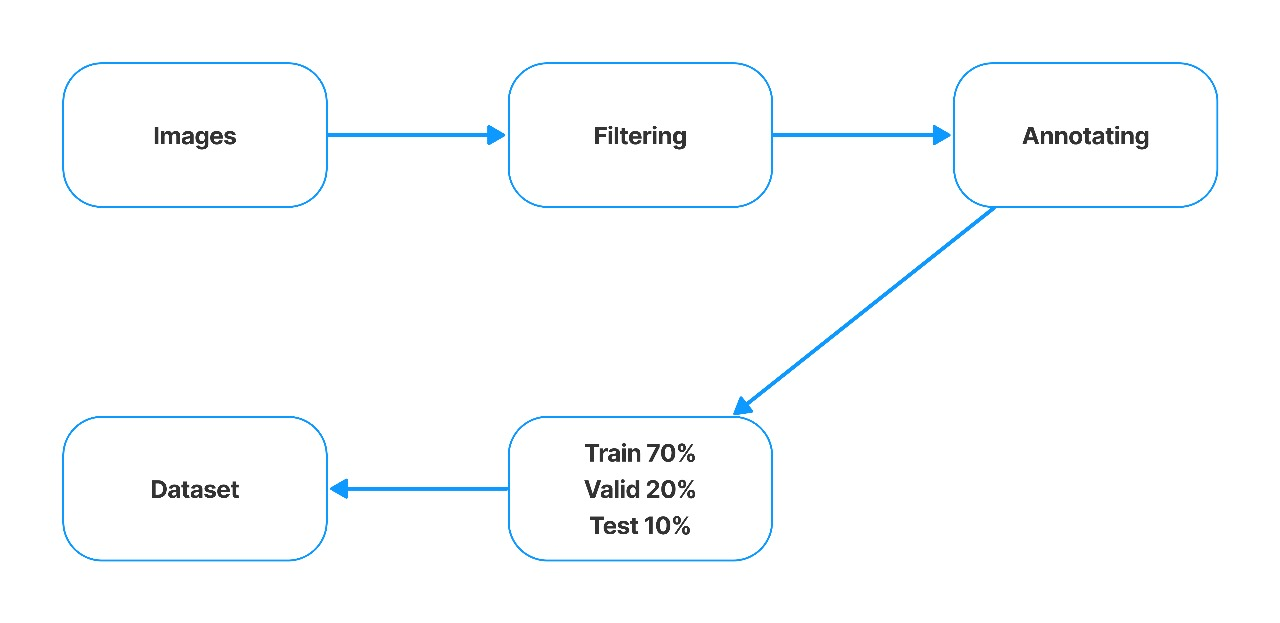
\includegraphics[width=0.5\textwidth, height=7cm]{images/block.jpeg}  % Adjust width and height
\caption{Block Diagram Dataset Creation.}
\label{fig}
\end{figure}


\subsection{Model Architecture}
The AI-based offline exam proctoring system utilizes a specific model architecture.At the forefront of the YOLO series, YOLOv8 is distinguished by its real-time accuracy and intricate design, which blends spatial attention modules with convolutional neural networks (CNNs) for improved feature identification [13]. The 53 convolutional layers that make up the CSPDarknet53 backbone are key to its design; they effectively maximize feature extraction, which is important for identifying the students in the examination hall . YOLOv8 is suited to different processing requirements and comes in nano to extra- large configurations. The medium to extra-large variants are beneficial for detecting the students more accurately.
\usepackage{graphicx} % Assuming graphicx is already loaded

\begin{figure}[htbp]
\centering
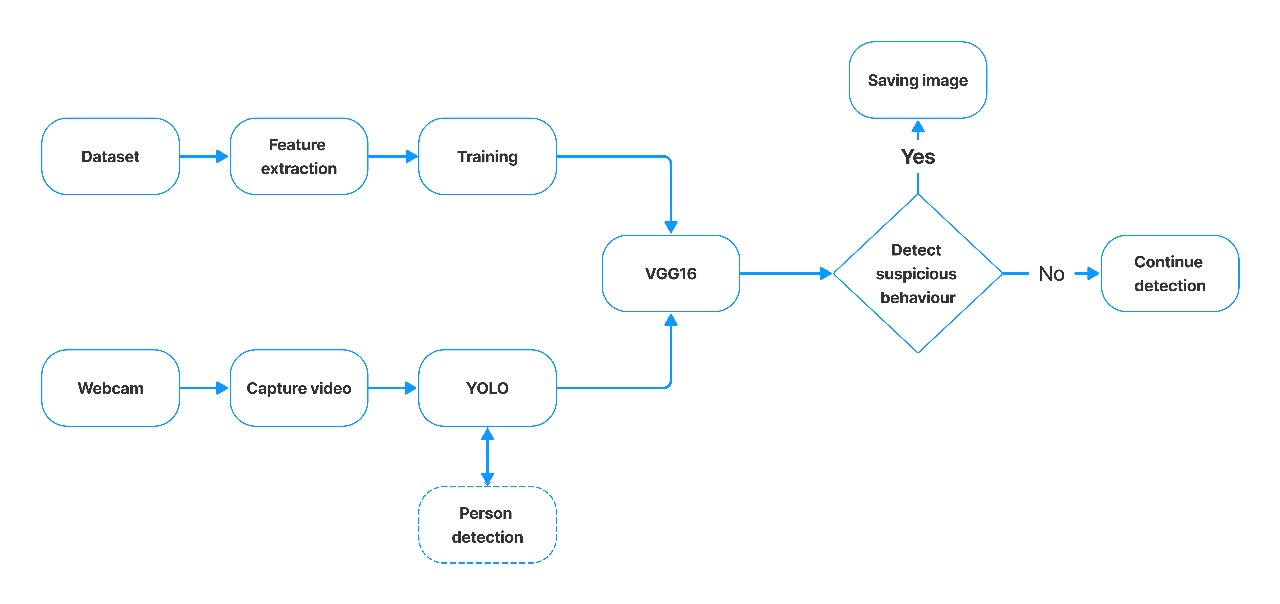
\includegraphics[width=0.5\textwidth, height=9cm]{images/ARC.jpeg}  % Adjust width and height
\caption{Block Diagram of Proposed System.}
\label{fig}
\end{figure}

For the classification of data, the VGG-16 Classifier has been employed. This classifier is known for its effectiveness in accurately categorizing various types of data. By utilizing this classifier, the system can efficiently determine whether a given frame falls under the "cheating" or "not cheating" category.

To ensure consistency and compatibility, the input frames are standardized to a size of 224 pixels by 224 pixels. This standardization allows for seamless processing and analysis of the frames, enabling the system to effectively detect any instances of cheating during the exam.


\subsection{Model Training}
The design of the offline exam proctoring system utilizing artificial intelligence has been structured to ensure efficient monitoring and supervision during examinations. This model architecture incorporates advanced AI technology to detect and prevent any form of cheating or misconduct during offline exams.

YOLOv8 pre-trained on COCO dataset, enabling it to learn and generalize patterns by exposing it to real-time environment. The Convolutional Neural Network (CNN) backbone serves as a feature extractor,learning essential patterns from input images.

A VGG16 Image classifier trained on a custom dataset to identify the "cheating" and "non-cheating" behaviour. The transfer learning technique is used in the classifiers training to reduce the time and effort to train the classifier.
\begin{table}[htbp]
\caption{VGG16 Classifier}
\label{tab2} % Label for referencing later
\begin{center}
\begin{tabular}{|c|c|}
\hline
\textbf{VGG16 parameters} & \textbf{parameter values} \\ % Bold headers
\hline
Batch size & 32 \\ % Second row
\hline
Epochs& 50 \\
\hline
Optimizer& adam\\
\hline
Class mode& Categorical\\
\hline
loss & categorical\_crossentropy \\

\hline
%\multicolumn{2}{l}{$^{\text{a}}$Footnote text here.} % Footnote
\end{tabular}
\end{center}
\end{table}





\subsection{Object Detection}
The video feed of the exam environment is segmented into a grid of cells, and employing a YOLOv8-like methodology, the object detection model detects students within each cell. This grid-based methodology enables the system to perform simultaneous monitoring of the entire exam setting, facilitating comprehensive detection coverage throughout the entirety of the video feed.

\begin{figure}[htbp]
\centering
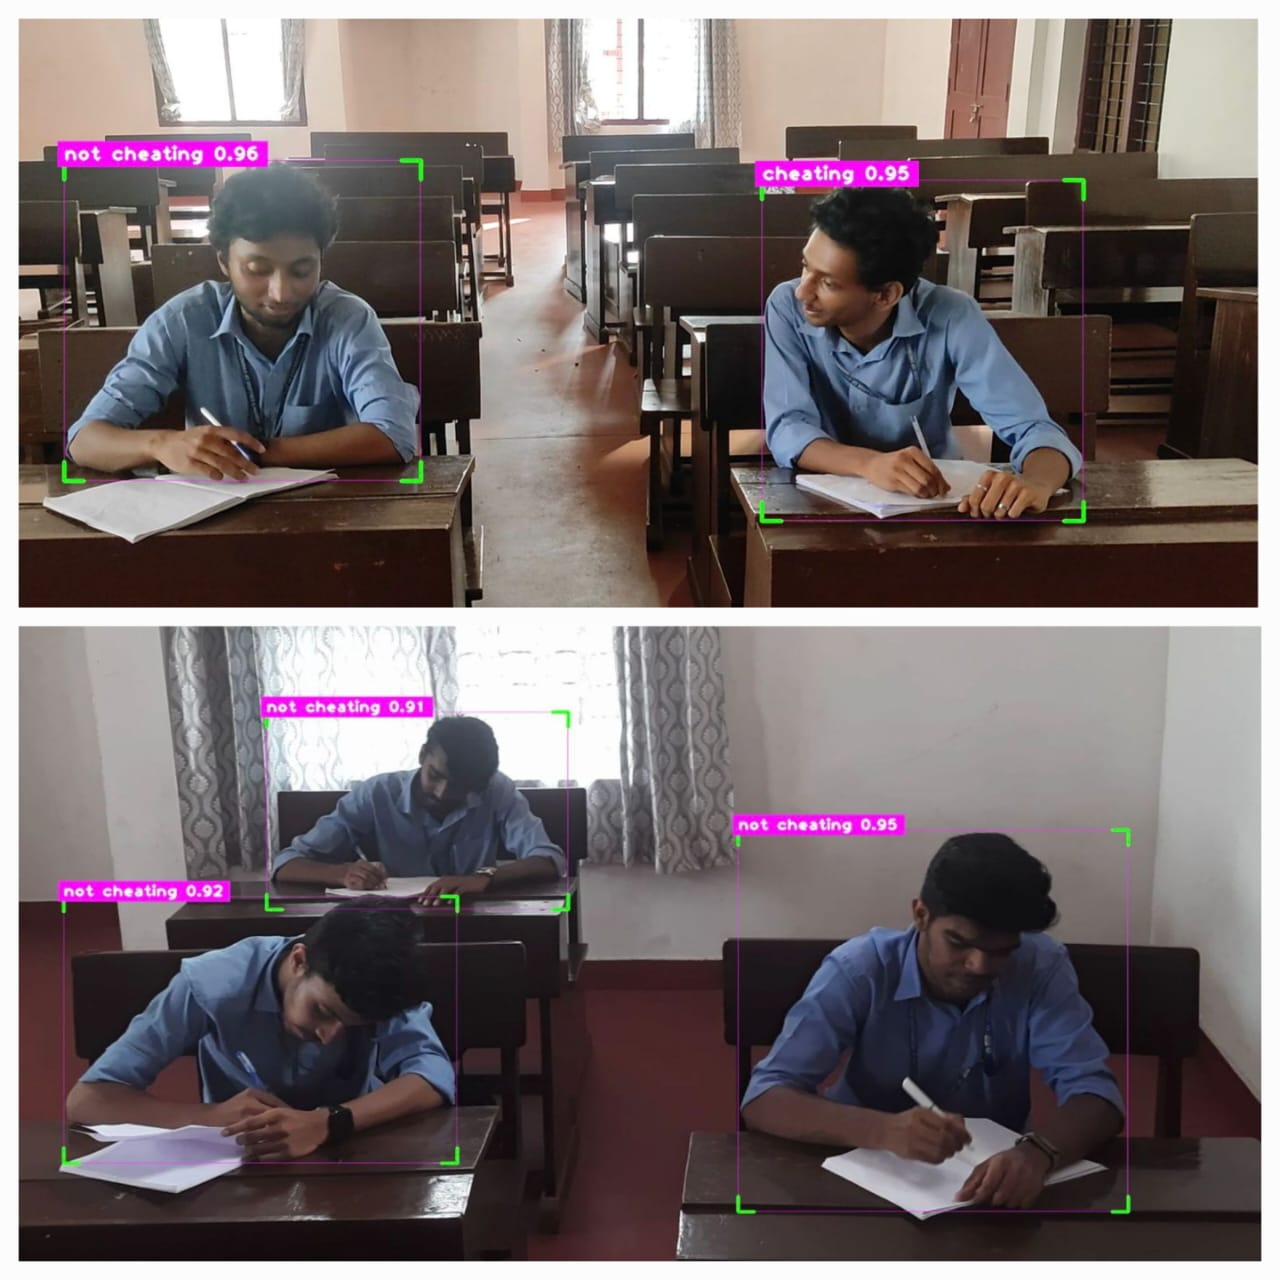
\includegraphics[width=0.5\textwidth, height=10cm]{images/detection.jpeg}  % Adjust width and height
\caption{Predicted Output From the Model}
\label{fig}
\end{figure}


\subsection{Classification}
The classification of offline exam proctoring systems has undergone a significant transformation with the integration of artificial intelligence (AI). By leveraging a dataset that has been meticulously annotated in roboflow, the system can effectively discern between the various behaviors displayed by students during exams using VGG16 classifier, specifically focusing on distinguishing between cheating and non-cheating actions.

\subsection{Output and Utilization}
 The utilization of offline exam proctoring system powered by AI not only promotes academic integrity but also improves the overall efficiency of the examination process. With AI technology, institutions can automate the monitoring and evaluation of exams, saving time for both educators and students. This streamlined approach enhances the productivity of exam administration while maintaining the quality and accuracy of assessments.

 Along with real-time detection, images of student who attempted to commit malpractices during the exam are also saved to a folder for later cross references with their confidence score.

\section{Implementation and Result}
\subsection{Implementation}
The study used an advanced object identification model called YOLOv8 (You Only Look Once version 8) to achieve real- time and accurate detection of students in the class. YOLOv8 is widely recognized for its remarkable precision and effectiveness in object recognition, rendering it a perfect match for the specific object detection task. The VGG16 classifies the images into required classes.

A centralized system with a good graphical processor act as the central hub of the entire system which houses an object detection model(YOLOv8)and an image classification model(VGG16)

\subsection{Performance Evaluation}
The result in Table II demonstrates that in the study of YOLOv8 for the detecting the students in exam hall, the model showed outstanding performance across key metrics.
YOLOv8 continuously maintained high precision, as seen by its high Mean Average Precision (mAP) , guaranteeing the accuracy of 95\% in detecting students. It minimized false positives with an exceptional precision score of 0.94. With closely no misses, the model’s recall of 0.96 demonstrated its ability to accurately identify all the  students .
All of these findings demonstrate how reliable and accurate YOLOv8 is an appropriate model to detect students in the classroom, which makes it an important tool for offline exam proctoring.YOLOv8 is the most trending and accurate model which has accuracy close to perfect predictions. combining the state-of-the-art YOLOv8 and VGG16 provided the project with a level of perfection that is unmatchable with humans.Humans has blind spots and other limitations but the EX-GUARD does not have such limitations.

The VGG16 classifier which was trained in house using our custom data set showed some of the best result.the trained model could adapt to the varying demands and situations of the examination hall.The VGG16 Provided an accuracy of 92\% in its evaluation phase.

\begin{figure}[htbp]
\centering
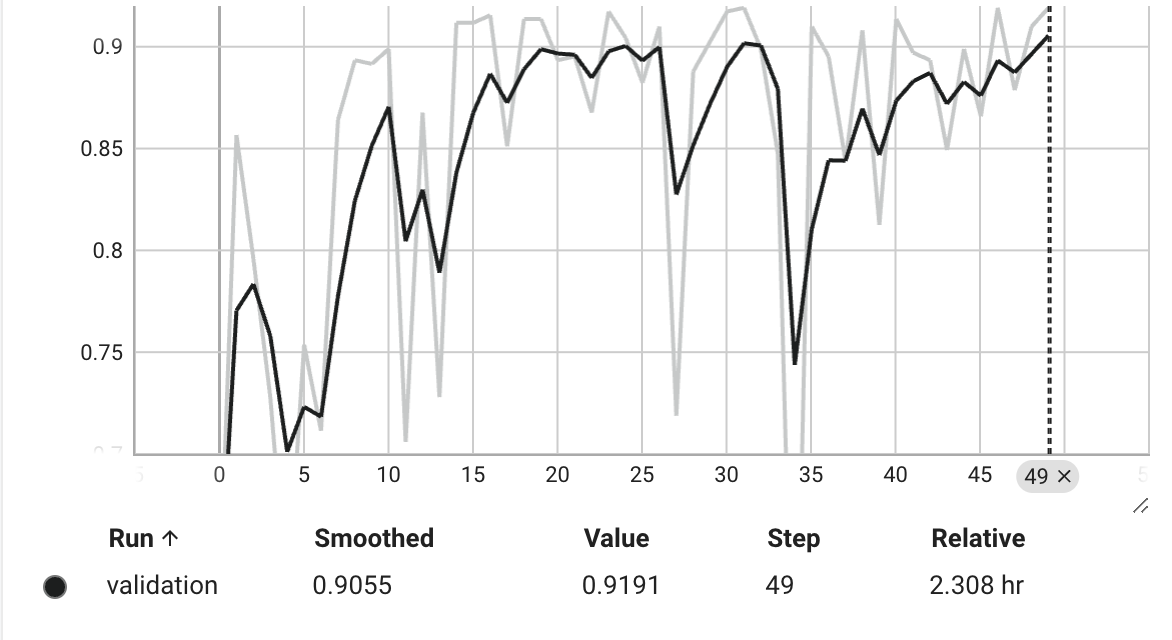
\includegraphics[width=0.5\textwidth, height=7cm]{images/Vgg16acc.png}  % Adjust width and height
\caption{Accuracy of Vgg16}
\label{fig}
\end{figure}

While comparing with other models like AlexNet, the VGG16 provided better output regarding the ability to classify the student's behaviors. Combining the YOLOv8 and VGG16 the system performed better than the humans. 




\begin{table}[htbp]
\caption{Performance Evaluation:YOLOv8}
\label{tab2} % Label for referencing later
\begin{center}
\begin{tabular}{|c|c|}
\hline
\textbf{Metric} & \textbf{YOLOv8} \\ % Bold headers
\hline
Accuracy & 95\% \\ % Second row

\hline
Precision&0.94\\
\hline
Recall&0.96\\
\hline
 F1-score&0.95 \\

\hline
%\multicolumn{2}{l}{$^{\text{a}}$Footnote text here.} % Footnote
\end{tabular}
\end{center}
\end{table}








\subsection{Findings}
From Fig. 6, which illustrates the usefulness of the YOLOv8
model for detecting students and VGG16 for classification, the study derives a number of noteworthy findings. The following are the main findings:
\begin{enumerate}
    \item  High detection Accuracy: The high Mean Average Precision (mAP) score indicates that the YOLOv8 model typically attained a high level of accuracy. This high accuracy ensures correct detection of exam takers.
    \item High classification accuracy: The high accuracy of VGG16 classifier(92\%) plays a major role in correctly classifying between cheating and non cheating.
     \item Precision and Recall: The model’s 0.94 precision and 0.96 recall scores
highlights its ability to reduce false positives, a crucial
aspect of detecting only students from each frame.
 
    \item Balanced F1-Score: At 0.95, the F1-Score, a measure of
accuracy that is balanced, was observed. This measure
shows that the YOLOv8 model successfully reduces false
positives and false negatives while maintaining good
detection accuracy.
\item Practical Deployment: We have developed a practical and
easily understandable automated proctoring system by integrating pre-trained YOLOv8 model with our custom-trained VGG16 classifier. 


\end{enumerate}


By providing a user-friendly interface for monitoring road
conditions, this system makes real-time analysis and reporting easier.

These indicate the resilience and effectiveness of the YOLOv8
model in detecting students and VGG16 model in classifying the students into "cheating" and "non cheating". The foundation for improved road maintenance and safety is laid by this research,
which may find use in damage prevention and real-time
monitoring.

\subsection{Comparison with State-of-the-Art methods}
In the realm of offline exam proctoring systems, leveraging deep learning models for real-time detection and analysis has become increasingly prevalent. This script integrates several state-of-the-art components, notably utilizing YOLO (You Only Look Once) for object detection, particularly focusing on identifying individuals, typically students, within an exam setting. YOLO offers real-time object detection with impressive accuracy, efficiently bounding boxes around detected objects. YOLOv8 is the best-performing object detection algorithm[17] in the field with the highest accuracy and performance measures.

the system also uses VGG16 classifiers for classifying images, we trained the  AlexNet with the same dataset as that of the VGG16. Referring to Table II, the following outcomes of the comparative study between VGG16 (the proposed model) and AlexNet on the same dataset are shown:
\begin{table}[htbp]
\caption{Comparison of the Performance Metrics for VGG16 and AlexNet}
\label{tab2} % Label for referencing later
\begin{center}
\begin{tabular}{|c|c|c|}
\hline
\textbf{Metric} & \textbf{VGG16} & \textbf{AlexNet} \\ % Bold headers
\hline
Accuracy & 92\% & 64\%\\ % Second row

\hline
Loss&68&76\\
\hline

%\multicolumn{2}{l}{$^{\text{a}}$Footnote text here.} % Footnote
\end{tabular}
\end{center}
\end{table}



\begin{figure}[htbp]
\centering
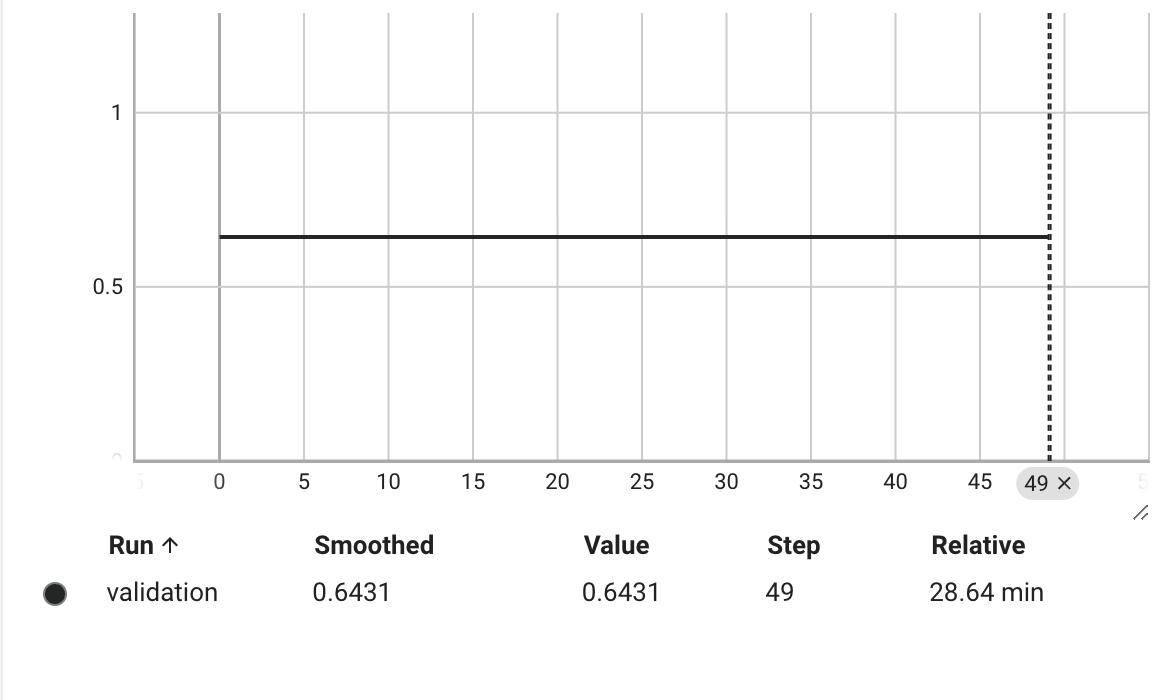
\includegraphics[width=0.5\textwidth, height=7cm]{images/AlexNet.png}  % Adjust width and height
\caption{Accuracy of AlexNet}
\label{fig}
\end{figure}



\section{Conclusion}
The offline exam proctoring system using AI is an utilization of a combination of YOLO object detection for detecting people in a video stream and a pre-trained VGG16 model for determining whether detected individuals are engaged in cheating behavior during an exam.

In essence, the system processes each frame of the video stream, identifying people using YOLO, and then analyzing each detected person's behavior using the VGG16 model. If the VGG16 model predicts that the person is potentially cheating based on certain features extracted from their behavior or surroundings, such as looking at unauthorized materials, it saves an image of the person for further review. Conversely, if the model determines that the person is not engaged in cheating behavior, it continues processing the video stream. This process is repeated for each frame of the video, allowing the system to continuously monitor and flag potential instances of cheating during an exam.

. 

\section*{References}
[1] Tong Liu ,AI proctoring for offline examinations with 2-Longitudinal-Stream
    Convolutional Neural Networks 10 December 2022
 
[2] Musa Dima Genemo ,Suspicious activity recognition for monitoring cheating in     exams 24 February 2022

[3] Fairouz Hussein , Ayat Al-Ahmad , Subhieh El-Salhi , Esra’a Alshdaifat ,         Mo’taz Al-Hami ,Advances in  Contextual Action Recognition: Automatic 
     Cheating Detection Using Machine Learning Techniques ,31 August 2022

[4] Rhitvik Pasricha ,Prathamesh Churi ,A Systematic Review on AI-based      
    Proctoring Systems: Past, Present  and Future September 2021
    
[5] Joseph Redmon, Santosh Divvala, Ross Girshick, Ali Farhadi You Only   
     Look Once: Unified, Real-Time Object Detection ,9 May 2016

[6] Tanzila Saba, Amjad Rehman, Nor Shahida Jamail1, SouadLarabi Marie-Sainte,
     Mudassar Raza, and Muhammad Sharif Categorizing the Students’ Activities for
     Automated Exam Proctoring using Proposed DeepL2-GraftNet CNN Network and ASO Based Feature Selection Approach, March 2021

[7]  M. Ghizlane, B. Hicham, and F. H. Reda, "A New Modelof Automatic and             Continuous Online Exam Monitoring,"in 2019 International Conference on 
     Systems of Collaboration Big Data, Internet of Things & Security
    (SysCoBIoTS), 2019, pp. 1-5.

[8]  Mabrouk, A.B., Zagrouba, E.: Abnormal behavior recognition for 
    intel-ligent video surveillance systems: a review. Expert Syst. Appl.
     91,480–491 (2018)

 [9]   He, H., Zheng, Q., Li, R., Dong, B.: Using face recognition to detect
    “Ghost Writer” cheating in examination. In: International Confer-ence on
    E-Learning and Games, pp. 389–397 (2018)

[10] D. Erhan, C. Szegedy, A. Toshev, and D. Anguelov. Scalable
     object detection using deep neural networks. In ComputerVision and Pattern Recognition (CVPR), 2014 IEEE Conference on, pages 2155–2162. IEEE, 2014.

[11] B. Hariharan, P. Arbelaez, R. Girshick, and J. Malik. Simultaneous               detection and segmentation. In Computer Vision–ECCV 2014, pages 297–312.         Springer, 2014.     

[12] Saba, T., Rehman, A., Jamail, N. S. M., Marie-Sainte, S. L., Raza, M.,\ &         Sharif, M. (2021).Categorizing the students’ activities for automated exam       proctoring using proposed deep L2-GraftNet CNN network and ASO based             feature selection approach. IEEE Access, 9, 47639–47656. https://doi.org/        10.1109/ACCESS.2021.3068223
[13]Ultralytics Accessed: 04.08.2023 [Online]
    Available: https://www.ultralytics.com/

\end{document}
